\chapter{Learning Words Like Humans Do: Syntactic Smoothing for Language Model Training}
\label{chapter:syntatic-smoothing}

While the Chapter 3 explored curriculum learning as a way to structure the input space and learning trajectory of a model, I now turn to a complementary question: \emph{how can internal representations themselves be shaped to better support generalisation—particularly for uncommon tokens?} Just as children benefit from structured exposure to language, they also rely heavily on syntactic cues to make sense of unfamiliar words. This chapter investigates how language models might likewise leverage structural signals to improve lexical generalisation.

One of the most striking capabilities of human learners is their ability to infer the meaning of unknown words from syntactic and semantic context; recall the example of the made-up word `zambled' from Chapter 2.

% Consider the sentence: ``the Golden Gate Bridge has been \emph{obnebulated} every morning this week, limiting visibility of the Pacific Ocean.'' Although most readers will not have encountered the word \textit{obnebulated}, we can make two confident inferences: (1) it is a verb, likely in the past participle form (given the ``has been'' auxiliary and the \textit{-ed} suffix), and (2) its meaning relates to fog or visibility. Human learners use this type of syntactic bootstrapping constantly.

This ability is notably lacking in current language models. Despite their success on many NLP benchmarks \citep{touvron2023llama, chowdhery2023palm}, pre-trained transformer language models still struggle with rare or unseen words. A key reason is that the vast majority of language models are pre-trained to maximise the log-likelihood of a word, given the surrounding context \citep{devlin2019bert, brown2020gpt3, chowdhery2023palm, touvron2023llama}. As language use is characterised by a Zipfian distribution \citep{zipf1935zipflaw}, language models are exposed to frequent tokens exponentially more often than infrequent ones during pre-training. Consequently, the representations of these frequent tokens are optimised based on exponentially more learning signals than those of low-frequency tokens. It has been shown that maximum likelihood objectives lead to representation degeneration in English language models because infrequent tokens are pushed into a narrow manifold of the representational space \citep{gao2018representation}. 

\begin{figure}[ht!]
    \centering
    \includegraphics[width=0.8\linewidth]{chapters/syntatic-smoothing/figures/anisotropy_visualization.pdf}
    \caption{Artistic visualization of the representational space of a language model, showing the clustering of tokens into a narrow manifold. The model is trained with a maximum likelihood objective, and the representations of the tokens are clustered together into a narrow manifold.}
    \label{fig:anisotropy_visualization}
\end{figure}

\newpage

This representation degeneration problem is linked to the broader phenomenon of anisotropy: the hidden states of a language model tend to cluster together into a small cone-shaped subspace, rather than over their full representational capacity \citep{arora2016latent, ethayarajh2019contextual, gao2018representation}. \cref{fig:anisotropy_visualization} illustrates this phenomenon. As language model evaluation is based on cumulative evaluation scores that conceal how well a model processes infrequent words, the disparities in the representational space are difficult to assess. This work makes two key contributions:

\begin{enumerate}
    \item First, this chapter introduces \smoothing, a simple but cognitively motivated method for improving the representation of infrequent tokens during language model training.\footnote{Code available at: https://github.com/rdiehlmartinez/syntactic-smoothing.} Inspired by the human tendency to group unknown words with structurally similar known words, I propose redistributing part of the learning signal for each token across other tokens that share similar syntactic roles. Using this method, tokens that are seldom seen during training benefit from the more frequent updates of tokens that occur in similar syntactic functions.  In effect, infrequent tokens benefit from updates to their syntactic neighbors, allowing them to ``learn by association'', as children often do.
    \item Next, I quantify the impact of this approach using a new diagnostic measure of \textbf{frequency bias}: a model's tendency to prefer grammatical sentences that contain high-frequency tokens over those with low-frequency ones. I then show that \smoothing reduces both frequency bias and anisotropy, without hurting performance on downstream tasks. These findings suggest that small structural changes rooted in cognitive observations can meaningfully improve the robustness and generalisation of small models.
     
\end{enumerate}

The remainder of this chapter is organised as follows: \cref{sec:anisotropy-background} goes beyond the background chapter and reviews the relationship between frequency and anisotropy in language models. Building on this background, \cref{sec:freq-bias} introduces the frequency bias metric that I propose to quantify the degree to which a model relies on frequency information over linguistic generalisation. \cref{sec:smoothing-method} introduces the \smoothing method and details its implementation. \cref{sec:results} both presents the results and analysis across synthetic and real-world evaluations and discusses the implications of these findings. Finally, \cref{sec:conclusion} summarises this work and motivates further exploration of how language models internalise linguistic structure over time.

\section{Anistropy}
\label{sec:anisotropy-background}


Through maximum likelihood training, language models implicitly learn to encode token frequency statistics. This training process gives rise to a frequency bias in models that constrains their ability to generalise to infrequent tokens. In this chapter, I will describe how this training process leads to a phenomenon known as anisotropy in language models' representational space. Before doing so, in this section, I describe more concretely how anisotropy is defined and how it is measured.

% \subsection{Generalization to Infrequent Tokens}

% Current approaches to language modeling rely heavily on the memorisation of infrequent tokens to perform well on downstream tasks \citep{feldman2020does}. Recent analytical work has shown that certain layers of transformer models implicitly store memorised long-tail data \citep{haviv2023understanding, kobayashi2023transformer}. \citet{feldman2020neural} demonstrate that models memorise atypical examples to achieve the highest accuracy on long-tailed data samples. This memorisation hack, however, has only been shown to work well with over-parameterised models \citep{belkin2019reconciling}. While these studies present various metrics to evaluate memorisation, these metrics do not capture how memorisation impacts generalised linguistic understanding within the models. In our work, we address this gap by developing a metric that quantifies the extent of this frequency bias in relation to models' linguistic abilities.

% Language use follows a Zipfian distribution, meaning that many tokens appear infrequently. Standard training objectives often require large models and noisy datasets with sufficient long-tail samples for effective generalisation \citep{zheng2022memorization}. However, improving generalisation without excessive scaling can be achieved by training models with inductive priors that leverage linguistic information. On the lexical level, the integration of morphological and orthographic information during representation learning has been explored to obtain more fine-grained word embeddings \citep{salle2018incorporating, vulic2017morphfitting, cotterel2015morphological, bhatia2016morphological, botha2014compositional}. To improve syntactic generalisation, the objective function has been enriched with auxiliary tasks, such as predicting constituency labels \citep{wang2023language}, hypernyms \citep{bai2022better}, dependency tags \citep{cui2022lert}, and POS tags \citep{diehlmartinez2023climb}. Some approaches have also shown promising results on rare word performance by constructing token embeddings that consider a word's surface form and surrounding context \citep{schick2019attentive, schick2020rare}.

\subsection{Anisotropy in Representational Space}
While frequency bias and generalisation capabilities can be observed by analysing model behavior on input--output patterns, representational analyses indicate that these phenomena are linked to the distribution of token representations. Language models trained as likelihood maximisers have been shown to yield degenerate representations for rare tokens \citep{gao2018representation}. Throughout training, infrequent tokens are disproportionately pushed in the negative direction of most hidden states, resulting in their clustering together irrespective of their semantic or syntactic properties. This clustering behavior leads to anisotropy: rather than occupying a large region of the representational space, token representations lie along a narrow manifold \citep{gao2018representation, ethayarajh2019contextual}

\subsection{Defining Anisotropy}

Anisotropy is defined as the inverse of isotropy: $1-I(v(\cdot))$. A representational space is isotropic if all the vector directions are distributed uniformly, meaning no particular direction is favored over another.

\citet{arora2016latent}\ and \citet{mu2018all} define isotropy as:

\begin{equation}
    I(v(\cdot)) \coloneq \frac{\min_{\norm{c}=1} Z(c)}{\max_{\norm{c}=1} Z(c)}
\end{equation}
where $c$ is a unit vector and $Z(c)$ is defined as the partition function over all tokens $w$ in the vocabulary $V$ , with representations $v(w)$:
$$
    Z(c) = \sum_{w \in V} \exp(c^Tv(w))
$$
In practice, this definition of isotropy is analytically infeasible to solve. In this chapter, I follow an empirical approximation proposed by \citet{ethayarajh2019contextual}: 
\begin{equation}
\label{eq:empirical-isotropy}
    I(v(\cdot)) \coloneq \mathbb{E}_{i\ne j}\big(1-\cos(v(w_i), v(w_j))\big)
\end{equation}
Here, $w_i$ and $w_j$ are two tokens sampled from the vocabulary, and $\cos$ is defined as taking the cosine similarity of the two word representations for $w_i$ and $w_j$.  

Despite its prevalence, the impact of anisotropy on a model's language understanding abilities remains unclear. Some studies suggest that reducing anisotropy improves performance on non-contextual benchmarks, sentence comparison tasks, and multilingual benchmarks \citep{bis2021too, su2021whitening, rajaee2022isotropy}. Conversely, other research indicates that higher anisotropy might enhance semantic clustering tasks and that reducing anisotropy does not uniformly improve performance on common NLU tasks \citep{ait2023anisotropy, ding2022isotropy}. Furthermore, the relationship between anisotropy and maximum likelihood training has been questioned. Some researchers argue that isotropy exists in local manifolds of contextual word representations \citep{cai2020isotropy}, while others contend that anisotropy arises from the learning dynamics of the query and key attention matrices in transformer models \citep{godey2024anisotropy}.

% \subsection{Reducing Anisotropy}

% Existing methods to reduce anisotropy broadly fall into three categories. The first group of approaches transforms the hidden states of language models to remove semantically uninformative directions and to preserve the dimensions of maximal isotropy \citep{arora2016simple, mu2018all, raunak2019effective, su2021whitening,bis2021too}. This intervention style is based on the assumption that the top singular dimensions of pre-trained word representations encode frequency statistics rather than semantic or lexical information \citep{mu2018all}. The second category of methods introduces novel training objectives and regularization terms that reduce the effects of anisotropy \citep{gong2018frage, gao2018representation, wang2019improving}. This type of approach places an inductive bias on representations that push the embeddings of frequent and infrequent words to occupy a similar semantic space. The third set of approaches explores different training paradigms to directly minimise anisotropy, such as using normalizing flow models \citep{li2020sentence} or manipulating the gradients used in maximum likelihood models \citep{yu2022rare}.

\vspace{1em}

While frequency bias and anisotropy are prevalent in language modeling, quantifying their effects and understanding their impact on generalisation, particularly for infrequent words, remains an open area of research. This chapter introduces a novel method for improving the representation of infrequent tokens by integrating linguistic information. Moreover, I hypothesise that adjusting the learning process to better represent infrequent tokens will also reduce anisotropy, as these two phenomena are interconnected.

\section{Frequency Bias}
\label{sec:freq-bias}

BLiMP is carefully balanced to ensure individual tokens occur equally in both sentence types. However, within a single pair, there may be an imbalance in average token frequency: For instance, the sentence
\textit{Grace's piano teachers are \textbf{known}} has a log frequency of 8.35 while its associated minimal pair \textit{Grace's piano teachers are \textbf{replied}} has a log frequency of 6.20.  I hypothesise that despite the minimal difference in BLiMP pairs, models trained in a typical manner will be biased by token frequency when determining grammatical acceptability.

\begin{wrapfigure}{r}{0.6\textwidth}
    \centering
    \includegraphics[width=0.6\textwidth]{chapters/syntatic-smoothing/figures/blimp_bias_example.pdf}
    \caption{Illustration of the BLiMP \textbf{frequency bias} calculation used to evaluate a model's reliance on frequency statistics when making predictions. The example BLiMP values are from a baseline RoBERTa model.}
    \label{fig:blimp_bias}
    \vspace{-1em}
\end{wrapfigure}

My goal is to quantify how language model performance differs between BLIMP pairs with large positive frequency differences (where the correct sentence has more frequently occurring tokens) and with large negative frequency differences (where the correct sentence has much less frequently occurring tokens). I do so in three steps.

First, I minimally preprocess BLiMP to ensure the analysis focuses on meaningful token-level differences. Specifically, I filter the dataset to only include sentence pairs where one set of tokens has been replaced by another set (e.g., ``The cat sat" vs ``The dog sat"). I exclude sentence pairs that differ only in token order (e.g., ``The cat sat" vs ``Sat the cat") or where tokens have been added to one sentence but not replaced (e.g., ``The cat sat" vs ``The cat sat quietly"). This filtering process removes approximately 15\% of the original BLiMP pairs and 9 of the 67 linguistic subtasks from consideration, but ensures that the frequency bias analysis focuses on genuine token-level substitutions that are most relevant for studying lexical generalisation.

Next, for each BLIMP sentence pair, I calculate the average (natural log) frequency of the differing tokens. Frequencies of individual tokens are computed with respect to a model's training data; for instance, in the example above the token \textit{\textbf{known}} has a log frequency of 8.35 in the training data. Sentence pairs are then ranked by the relative difference in these average frequencies, where positive values indicate a higher average frequency for the acceptable sentence. These relative differences form a distribution, as shown in the middle plot of \cref{fig:blimp_bias}. 

Then, I compute the BLiMP score using pseudo log-likelihood \citep{salazar2020masked} for BLIMP pairs in the upper and lower thirds of the relative frequency difference distribution. I exclude the middle third, as these represent pairs with minimal frequency differences (see the frequency plot for details). I define a model's \textbf{frequency bias} as the difference between the two BLiMP scores. The entire process is illustrated in \cref{fig:blimp_bias}. While the choice of partitioning the frequency pairs into thirds is somewhat arbitrary, I find that this division works well empirically; expanding the middle set of BLIMP sentences that I exclude would make the \textbf{frequency bias} more pronounced, but would lead to data sparsity. 

In practice, I find that standard transformer language models, such as OPT-125M \citep{zhang2022opt}, RoBERTa-base \citep{liu2019roberta}, and T5-base \citep{raffel2020t5}, exhibit a frequency bias as high as 13.7\%. My goal is to develop a model that can attain a frequency bias close to zero while attaining a high BLiMP score: that is, a model that makes determinations on the grammatical acceptability of sentences based solely on relevant linguistic aspects, rather than relying on possibly misleading statistical artifacts of the training data. 

\section{Syntactic Smoothing}
\label{sec:smoothing-method}

I hypothesise that transformer language models exhibit a strong frequency bias due to their maximum likelihood training objective, which limits infrequent tokens from receiving useful learning signals and thus hinders their ability to effectively encode linguistic information. To address this, I propose at each learning step to backpropagate the learning signal of a target token to all other tokens serving similar syntactic roles; this benefits infrequent tokens that appear less often in the training data.

\smoothing implements this strategy by distributing a portion of every update signal to all syntactically similar tokens using a syntactic similarity metric (operationalised below). This results in the representation of infrequent tokens approaching the average representation of all tokens that serve a similar syntactic function; e.g., the representation of a niche word like `obnebulated' would encode its syntactic role as a verb.

The \smoothing method consists of two components; (1) a similarity metric that uses part-of-speech distributions as a coarse proxy for syntactic similarity, and (2) an adjustment to the loss function to smooth the backpropagation signal over syntactically similar tokens during pre-training. 

\subsection{Syntactic Similarity Score}
\label{sec:sim}

The syntactic similarity between two tokens can be measured in multiple ways, e.g., by using surface features, dependency labels, or even the predictions of a teacher language model \citep{hinton2015distilling}. Here, I present a simple measure that acts as a coarse approximation for syntactic similarity: I consider two tokens to be similar if they have a similar distribution of part-of-speech tags in the training set.

I evaluate the syntactic similarity between tokens prior to training, as a one-off preprocessing step over the entire training set. First, I use the part-of-speech (POS) tagger from the NLTK package \citep{bird2009natural} to assign each word in the training set to one of 12 universal POS tags, based on its given context \citep{petrov2012universalpos}.\footnote{The 12 tags in the NLTK tagger are given here: \url{https://www.nltk.org/book/ch05.html\#tab-universal-tagset}. They are derived from the 17 tags in the Universal Dependencies tagset.} I then tokenise the training data into sub-word tokens and assign each token the POS tag corresponding to the word it belongs to in each instance. As words can take on a different part of speech depending on the context, I count the number of times each token in the vocabulary $V$ appears as each POS tag in the training data, producing a 12-valued vector. This results in a matrix $M \in \mathbb{R}^{|V|\times 12}$ containing the distribution over POS tags for each token. Finally, I can compute the similarity of two tokens $V_i$ and $V_j$ using the cosine similarity of their POS distributions: $$ \text{Syntactic Similarity(i, j)} = \frac{M_i^TM_j}{||M_i|| \cdot ||M_j||}$$ 


Note that while in this chapter I define syntactic similarity via cosine similarity, any real-valued distance metric or divergence can be used. The similarity function does not need to be symmetric, although I note that symmetric functions provide computational advantages as only half the values need to be computed and stored. Also, note that this methodology does not depend on a specific choice of POS tagger.

I provide the POS distributions and similarity distributions for the example tokens ``blind'' and ``the'' in \cref{fig:distributions}. Notice that ``the'' occurs almost exclusively as a determiner and is not similar to many other tokens, whereas ``blind'' occurs as a noun, verb, adjective, and adverb and has a high similarity to more than half the other tokens in the vocabulary.

\begin{figure}[ht!]
    \centering
    \includegraphics[width=0.8\linewidth]{chapters/syntatic-smoothing/figures/distributions.png}
    \caption{Part-of-speech distributions and similarity distributions for the subword tokens ``blind'' and ``the''. Similarities are computed as cosine-similarities against every other token in the vocabulary and sorted.}
    \label{fig:distributions}
    \vspace{-1em}
\end{figure}

\subsection{Smoothing the Backpropagation Signal}\label{section:smoothing}

Modern pre-training objectives implement likelihood maximisation using a cross-entropy loss between the label of the correct word and predicted probabilities from a forward pass of the model. \smoothing makes a small adjustment. Instead of a one-hot encoding, the target vector $t$ becomes a distribution across the entire vocabulary with some of the signal on the correct label $j$ and the rest of the signal distributed across all other tokens $i$ according to the syntactic similarity metric used:

\begin{equation}
\label{eq:signal-distribution}
    t_i=\left\{
  \begin{array}{@{}ll@{}}
    (1-\alpha), & \text{if}\ i=j \\
    \frac{s(i,j)}{\sum_{k=0}^{|V|}{s(i,k)}} \times \alpha & \text{otherwise}
  \end{array}\right.
\end{equation}

\noindent

where $\alpha$, the smoothing parameter, determines the proportion of the error signal reserved for the correct word and $s$ is the part-of-speech similarity metric. I experiment with different values for $\alpha$, noting that $\alpha=0$ is the standard likelihood maximisation task. I also investigate the use of a pacing function that linearly decreases $\alpha$ so that at the start of training the majority of the signal is propagated to other syntactically similar tokens and by the end of training nearly all of the error signal is sent to the correct token to ensure that the model still optimises perplexity. 

In practice, I also find it beneficial to apply a temperature scaling function to the syntactic similarity distribution. Thus, rather than using the raw syntactic similarity scores, $s(i,j)$, in \cref{eq:signal-distribution}, I use the temperature-scaled similarity scores:

$$
s'(i,j) = \frac{\exp\left(\frac{s(i,j)}{\tau}\right)}{\sum_{k=1}^{|V|} \exp\left(\frac{s(i,k)}{\tau}\right)}
$$
where $\tau$ defines the temperature which I set to $\tau=0.025$.

\subsection{Experimental Setup}
\label{subsection:experimental_setup}

These experiments focus on smaller language models and datasets due to computational constraints and the particular challenges of generalizing to uncommon instances under resource-constrained training conditions \citep{warstadt2023babylm1}. 

\paragraph{Data} \label{paragraph:data} As in Chapter 3, I use the same dataset published as training data for the BabyLM challenge at the 2023 CoNLL workshop \citep{warstadt2023babylm1}. The dataset is pre-processed in the same way as in the previous chapter. 

\paragraph{Model} Similarly, the model used for these experiments is the same as the one in Chapter 3: a small 8-layer encoder-style RoBERTa model with pre-layer normalization \cite{huebner2021babyberta}; hyper-parameters, choise of tokeniser (BPE tokeniser) and vocabulary size are all the same. 

\paragraph{Evaluation} I evaluate the BLiMP frequency bias of the models, as defined in \cref{sec:freq-bias}, on the evaluation set of BLiMP. To compute anisotropy I use the formulation defined in \cref{eq:empirical-isotropy}; I sample 1,000 pairs of random word tokens with their surrounding context from the training set, and compute the cosine similarity of their hidden representation at each of the 8 layers of the RoBERTa model. To obtain a model's final anisotropy value, I average the anisotropy scores across the 8 layers. Additionally, I finetune and evaluate each model on two downstream sentence-level tasks, COLA \citep{warstadt2019cola} and SST-2 \citep{socher2013sst}, as well as two language inference tasks, MNLI \citep{williams2018mnli} and QNLI \citep{rajpurkar2016squad, wang2018glue}.


\paragraph{Baselines}

I introduce three types of baselines: 
\begin{enumerate}
    \item \textbf{Popular open-source transformer models}: OPT-125M \citep{zhang2022opt}, RoBERTa-base \citep{liu2019roberta}, and T5-base \citep{raffel2020t5}, pre-trained from scratch on the same dataset I describe in \cref{subsection:experimental_setup}. I use the default configuration for each model resulting in a varied number of parameters.
    \item \textbf{Base Model}: The small RoBERTa model described above without \smoothing.
    \item \textbf{Label Smoothing}: The base model trained with label smoothing \citep{szegedy2016rethinking}. I train a baseline with a low-level of smoothing ($\alpha=0.2$) and a mid-level of smoothing ($\alpha=0.5$). Note that \smoothing can be seen as a linguistically-guided version of the standard label smoothing approach, in which the learning signal is distributed to all tokens uniformly.
\end{enumerate}


\paragraph{Models} I train all models with \smoothing using the same two $\alpha$ values as the label smoothing baselines to facilitate comparison. I also run variants using the linear pacing function presented in \cref{section:smoothing} which linearly decreases the smoothing from an initial value of $\alpha$ to zero across training. For these variants, I use the same two values of smoothing, as well as an additional high value of $\alpha=0.8$ giving a total of five \smoothing variants. I do not include unpaced \smoothing with a high value of $\alpha$ as initial experiments found that distributing such a high proportion of the learning signal away from the correct token leads to high perplexity and poor downstream performance.

\section{Results}
\label{sec:results}

\begin{table*}[ht!]
    \centering
    \small
    \setlength{\tabcolsep}{4pt}  % Reduce column spacing
    \begin{tabular}{ll||cc|ccccc}
    \toprule
    \textbf{Model}  & $\alpha$ & \textbf{Bias}  & \textbf{Anisostropy} & \textbf{BLiMP} & \textbf{COLA} & \textbf{SST-2} & \textbf{MNLI} & \textbf{QNLI}  \\
    \midrule
    OPT   & - & 10.6 & - & 63.2 & 64.6 & 81.9 & 57.6 & 61.5\\
    RoBERTa & - & 13.7 & - & 69.8 & 70.8 & 87.0 & 73.2 & 77.0\\
    T5      & - & 6.2 & - & 58.3 & 61.2 & 78.1 & 48.0 &  62.0\\
    \midrule
    \midrule
    Base Model & -&9.8 & 51.3 & 71.4 & 71.4 & 82.9 & 69.6 & 79.7 \\
    \midrule
    \multirow{2}{*}{\makecell[l]{\texttt{Label}\\\texttt{Smoothing}}} &Low & 5.5 & 40.2 & 73.2 & 70.7 & 84.0 & \textbf{70.1} & 80.0 \\
    &Mid & 2.7  & 40.3 & 73.0 & 71.5 & 82.2 & 69.0 & 79.4 \\
    \midrule
    \multirow{5}{*}{\makecell{\texttt{Syntactic}\\\texttt{Smoothing}}}&Low  & 2.9 & 39.7 & \textbf{73.2} & 70.7 & 84.9 & 69.7 & 79.2 \\
    &Mid  & \textbf{-0.2} & 33.8 & 72.1 & \textbf{71.9} & 83.5 & 67.2 & 79.4 \\
    &P. Low & 7.4 & 39.9 & 71.9 & 70.5 & \textbf{85.2} & 70.0 & \textbf{80.4}\\ 
    &P. Mid& 5.7 & 34.5 & 72.3 & 71.8 & 84.0 & 68.2 & 78.9\\ 
    &P. High & 5.2 & \textbf{31.0} & 72.2 & 70.5 & 83.7 & 67.7 & 79.1 \\ 
    \bottomrule
    \end{tabular}
    \caption{\label{tbl:full-results} I report bias~($\downarrow$), anisotropy~($\downarrow$), BLiMP~($\uparrow$) score, and accuracy or correlation scores ($\uparrow$) on two downstream sentence-level tasks -- COLA and SST-2 -- and two downstream language inference tasks -- MNLI and QNLI -- for the MLM baseline, two label smoothing (LS) baselines, and five \smoothing variants. Paced (P. Low, Mid, High) variants use linear pacing to reduce the smoothing factor to zero over training.}
\end{table*}

The results are summarised in \cref{tbl:full-results}. I find that the method reduces frequency bias while retaining strong language modeling capabilities. At the same time, I observe that the models with the lowest frequency bias also demonstrate the lowest anisotropy. I then extend the analysis beyond the specific phenomenon of frequency bias and anisotropy by examining the impact of \smoothing on the linguistic generalisation capabilities of the model and its downstream performance after finetuning. Finally, I find that an alternative syntactic scoring metric leads to similar results as the cosine-based definition.

\subsection{Anisotropy and Frequency Bias}

\begin{wrapfigure}{r}{0.5\textwidth}
    \centering
    \includegraphics[width=0.5\textwidth]{chapters/syntatic-smoothing/figures/biases.png}
    \caption{Frequency bias for the three open source models, the base model, the two label smoothing (LS) baselines and the two \smoothing (\texttt{SyS}) models.}
    \label{fig:biases}
\end{wrapfigure}

I conduct analyses to inspect the learning dynamics of my method and its effect on frequency bias and anisotropy in more detail. 

\paragraph{\smoothing reduces a model's frequency bias.}
I find that all four pre-trained models exhibit strong frequency bias (see \cref{fig:biases}); they are more likely to incorrectly prefer ungrammatical sentences if they contain tokens that occur more frequently during training. This confirms the hypothesis that the evaluation of generalisation capabilities is obfuscated by frequency effects. 

By contrast, the two \smoothing variants successfully reduce the frequency bias. The frequency bias is almost completely removed in the case of the \texttt{Mid} variant, which distributes exactly half of the training signal to syntactically similar tokens. I further observe that the Label Smoothing baselines also reduce bias but to a lesser extent than the corresponding \smoothing models with the same degree of smoothing. 


\paragraph{\smoothing reduces anisotropy.}

As shown in \cref{tbl:full-results}, \newline \smoothing reduces anisotropy over both the base model and label smoothing baselines.\footnote{Note that I do not compute the anisotropy for the three open-source pre-trained models (OPT, RoBERTa, T5) because these models use different architectural configurations than the models I train (e.g., larger hidden dimensions).} Label smoothing reduces anisotropy, but not to the same extent as the \smoothing models. To better understand how anisotropy develops in a model, I compute the model's anisotropy scores at eight checkpoints during training, as shown in \cref{fig:anisotropy-learing-dynamics}. I find that a greater degree of smoothing leads to a greater reduction in anisotropy for the \smoothing variants (it is less clear if this is the case for label smoothing), supporting the hypothesis that syntactic initialization helps promote better representation learning across the model's vocabulary. I also find that the pacing method leads to lower anisotropy than the flat method, with \texttt{SyS}-P (High) achieving the lowest anisotropy throughout.

\begin{figure}[ht!]
    \centering
    \begin{subfigure}[b]{0.49\textwidth}
        \centering
        \includegraphics[width=\textwidth]{chapters/syntatic-smoothing/figures/anisotropy-learning-dynamics.png}
        \label{fig:anisotropy-learing-dynamics}
    \end{subfigure}
    \hfill
    \begin{subfigure}[b]{0.49\textwidth}
        \centering
        \includegraphics[width=\textwidth]{chapters/syntatic-smoothing/figures/anisotropy-layers.png}
        \label{fig:anisotropy-layers}
    \end{subfigure}
    \caption{Anisotropy learning dynamics. \textbf{Left:} Comparison of the baseline RoBERTa model, two label smoothing (LS) baselines, and the \smoothing (\texttt{SyS}) models, with values in parentheses indicating the degree of smoothing. \textbf{Right:} Anisotropy learning dynamics across selected layers for the baseline and paced \texttt{SyS} model with high smoothing, highlighting the final layer difference at the end of training.}
    \label{fig:anisotropy-combined}
\end{figure}


Over the course of training, I observe a consistent double-dip trend: an initial dip followed by a sudden rise, followed by a second slow decrease in anisotropy. The \smoothing models do not see as large a sudden rise, maintaining a lower anisotropy throughout. To examine the learning dynamics in more detail, I also plot the evolution of the anisotropy across several layers of the baseline model and the \texttt{SyS}-P (High) variant, given in \cref{fig:anisotropy-combined}. Two observations stand out. The anisotropy of all layers in the \smoothing model is lower than in the corresponding layers in the baseline model across the entire learning process. In both the baseline model and the \smoothing model, earlier layers have lower anisotropy; this finding agrees with the same observation made by \citet{ethayarajh2019contextual}. Notably, in the final layer the anisotropy of the \smoothing model remains consistently low and does not increase significantly during training, in contrast to the drastic fluctuation observed in the baseline model. This is particularly interesting as the final layer is commonly used for finetuning in downstream tasks and is empirically found to encode more high-level semantic information than the earlier layers \citep{clark2019does}. 

\paragraph{Frequency bias and anisotropy are correlated.}

For each model, I compute the model's frequency bias and anisotropy at multiple training stages. I plot the learning dynamics of anisotropy and frequency bias in \cref{fig:bias-anisotropy-correlation}, only including the points after 50\% of training has been completed to avoid the noisy first dip observed in the anisotropy dynamics above. I find a positive Pearson correlation of 0.73 and a polynomial goodness-of-fit $R^2$ score of 0.63 between these two metrics.

It is also evident that the pacing approach re-introduces frequency bias towards the end of training, as the degree of smoothing is linearly reduced to zero. It is noteworthy that the final anisotropy and bias are lower than the baseline model, and completing training without any smoothing may be beneficial for downstream tasks, as explored in the next section.

\paragraph{Frequency Bias Disproportionately Affects Content Words}
\label{sec:word-class-versus-word-frequency}


To better understand the linguistic categories most impacted by frequency bias, I analyse the relationship between token frequency and syntactic class. Specifically, I compare the POS tag distributions of the top 100 most frequent tokens and the bottom 100 least frequent tokens in the training data. 

\begin{wrapfigure}{r}{0.5\textwidth}
    \centering
    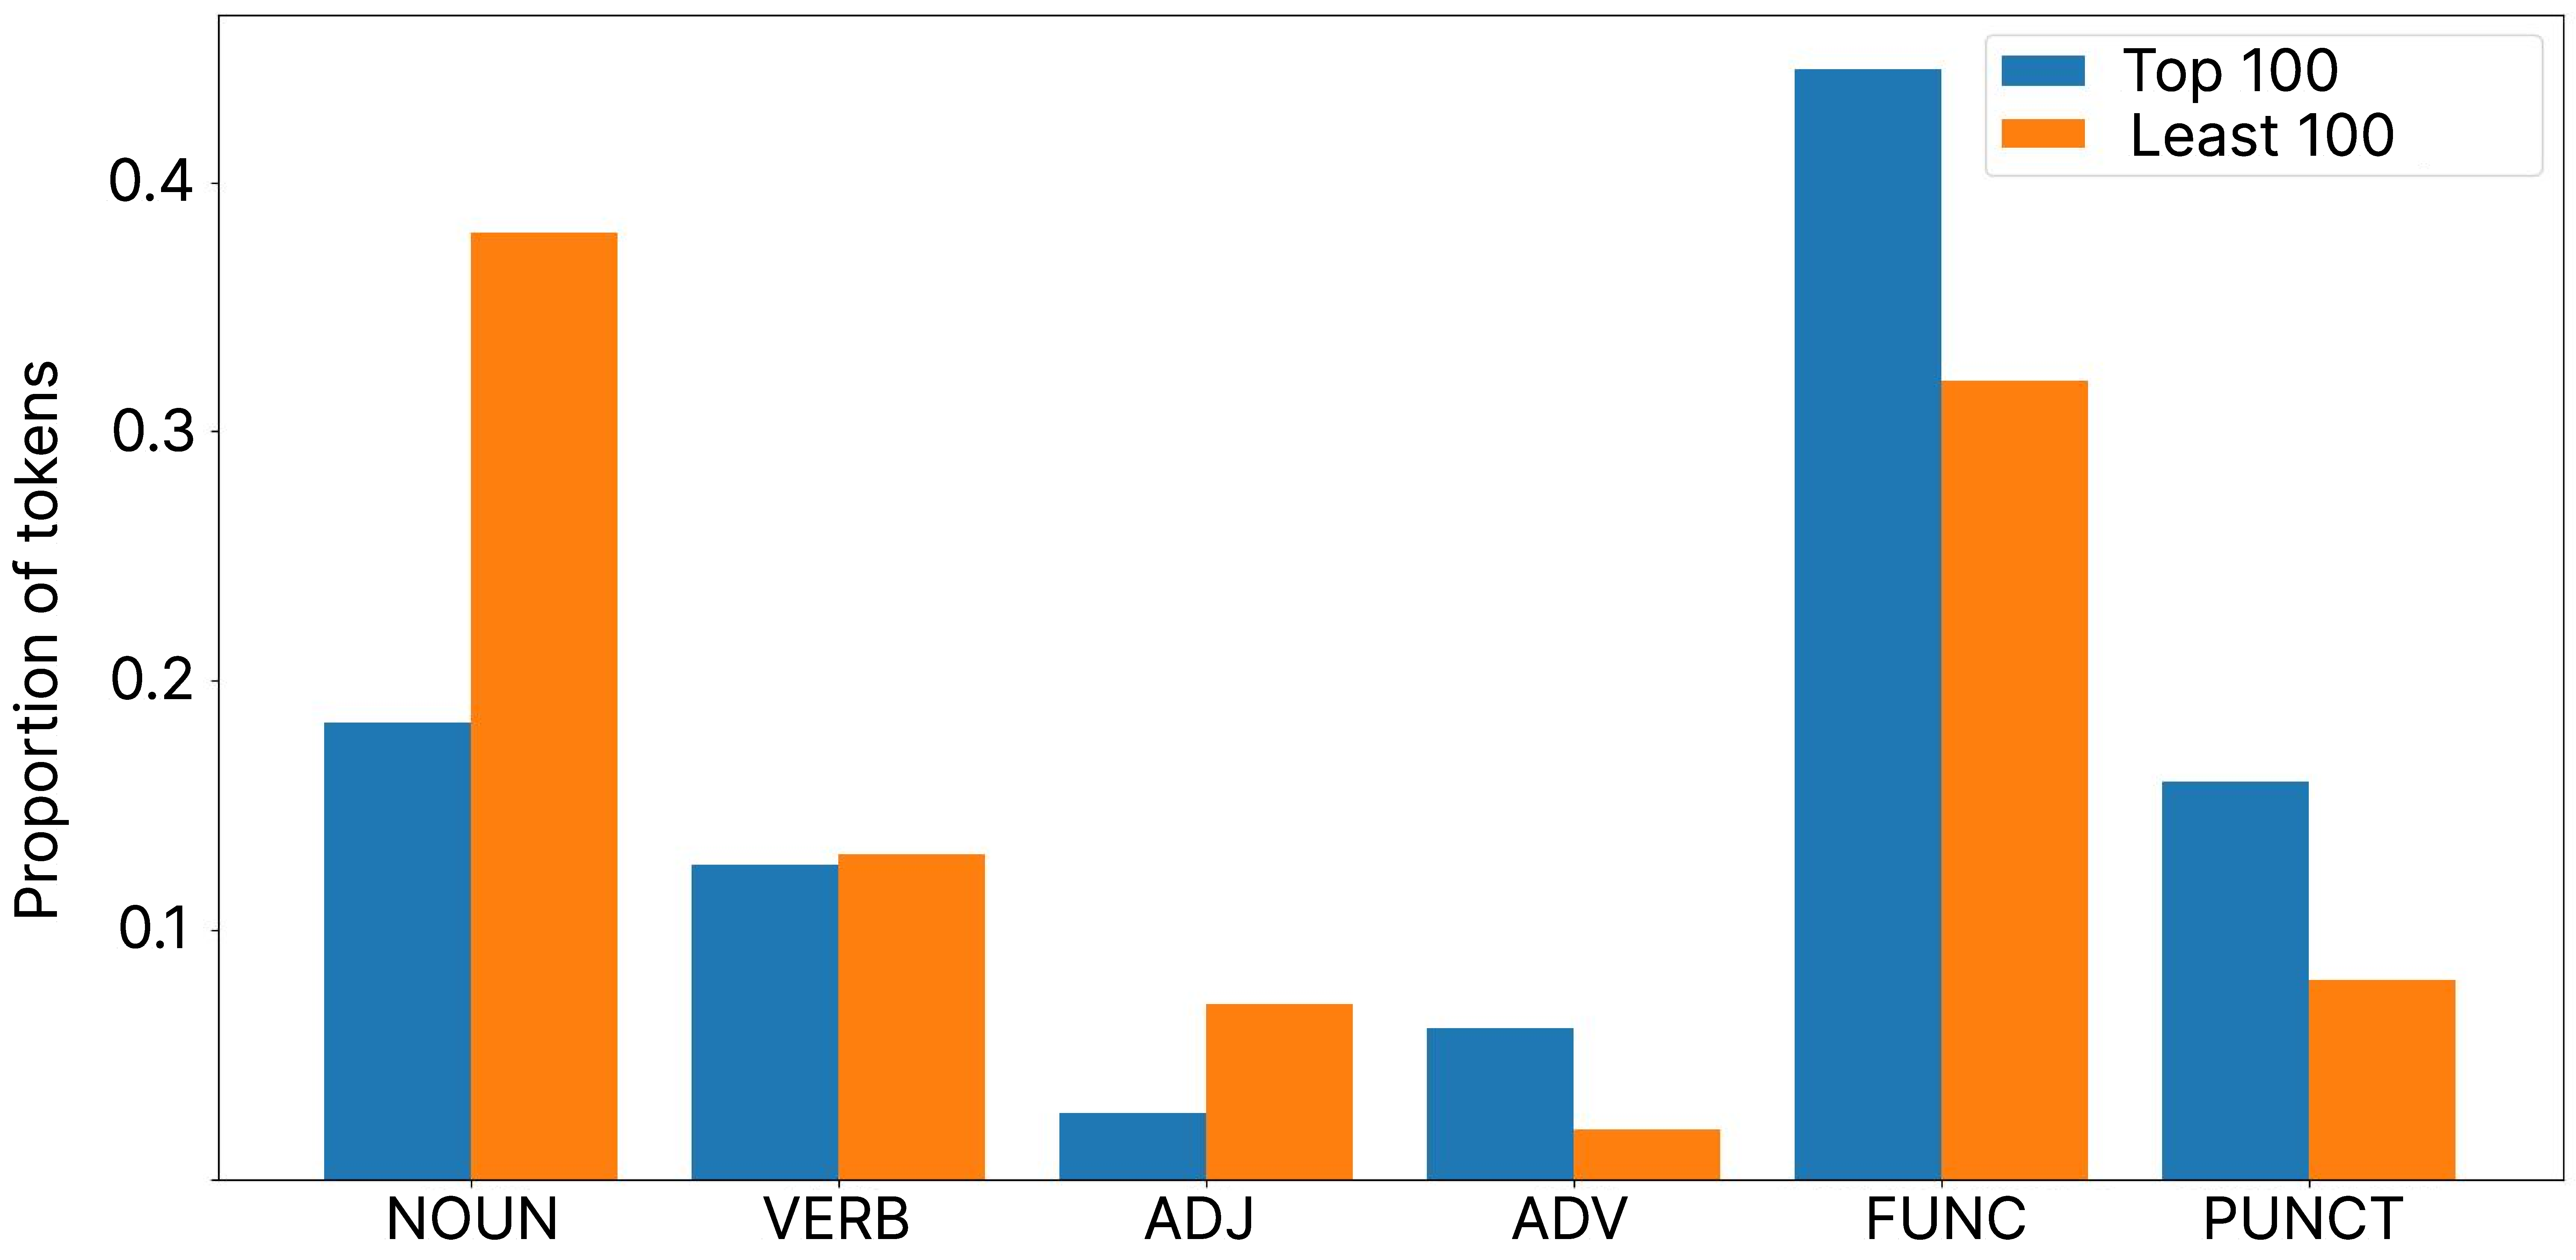
\includegraphics[width=0.49\textwidth]{chapters/syntatic-smoothing/figures/top_versus_bottom_pos_dist.pdf}
    \caption{Distribution across POS tags of the top \& bottom 100 most frequent tokens.}
    \label{fig:top-100-pos-dist}
\end{wrapfigure}

I find that content words, especially nouns, are over-represented in the low-frequency tail of the distribution, while function words dominate the high-frequency tokens. \cref{fig:top-100-pos-dist} illustrates this disparity. This suggests that frequency bias in language models may disproportionately hinder the learning of specialised vocabulary, particularly rare nouns and content-bearing expressions. It also reinforces the importance of a smoothing strategy that supports lexical generalisation by leveraging syntactic structure.

\begin{figure}[ht!]
    \centering
    \includegraphics[width=0.75\linewidth]{chapters/syntatic-smoothing/figures/bias-vs-anisotropy.png}
    \caption{Pairs of anisotropy, and frequency bias for the baseline RoBERTa model, the two label smoothing baselines and the \smoothing models. The arrows indicate increasing training progress (starting after 50\% of training has completed).}
    \label{fig:bias-anisotropy-correlation}
\end{figure}

\subsection{Effects of Smoothing on Downstream Tasks}
While the method primarily aims to enhance the representation of infrequent tokens, I sought to investigate the potential for improvement in standard evaluation measures, given the limited number of affected test instances. Nonetheless, I observe that all the \smoothing models, as well as the label smoothing models, achieve better BLIMP scores than the baseline model (see \cref{tbl:full-results}). These results suggest that methods that smooth label distributions, whether through a syntactic prior or a simpler uniform smoothing approach, enhance the representation of all tokens, including the more frequent ones.

I had concerns that softening the frequency bias with the smoothing methododology might lead to degraded performance in downstream tasks for which frequency can be a strong proxy. As a control condition, I finetune the model on two sentence-level tasks (COLA, SST-2) and two language inference tasks (MNLI and QNLI), both of which are part of the GLUE \citep{wang2018glue} benchmark. I find that none of the \smoothing objectives result in substantial performance degradation on these NLU tasks (see the last four columns of Table~\cref{tbl:full-results}), and in fact note that for some tasks, such as SST-2, the \smoothing models yield uniform increases in performance. While not comparable apples-to-apples, I report NLU performance for the open-source baselines in \cref{tbl:full-results} as a point of reference. 

\subsection{Alternative Measures of Syntactic Similarity}

In \cref{sec:sim} I define the syntactic similarity score that is used by the \smoothing approach as the cosine similarity between POS distributions. To examine how this specific choice of similarity metric impacts my approach, I replace the cosine-based definition with a Jensen Shannon-based definition:
$$ \frac{1}{2}\big[ \text{KL}(M_i, M_j ) + \text{KL}(M_j, M_i)\big],$$
where KL$(M_i, M_j)$ is the Kullback-Leibler divergence between the POS distributions, $M_i$ and $M_j$, for the vocabulary items $V_i$ and $V_j$.

\begin{table}[ht!]
\centering
\small
\begin{tabular}{l||cc|ccccc}
\toprule
\textbf{Model}  &  \textbf{Bias}  & \textbf{Anisotropy} & \textbf{BLiMP} \\
\midrule
Base Model & 9.8 & 51.3 & 71.4  \\
\midrule
\texttt{SyS} (Mid) \hspace{0.42cm} [JS]  & 3.6 & 34.7 & 71.3 \\
\texttt{SyS} (Low) \hspace{0.38cm} [JS]  & 4.1 & 34.6 & 73.3  \\
\texttt{SyS}-P (High) \hspace{0.05cm} [JS] & 6.6 & 36.7  & 72.5  \\ 
\texttt{SyS}-P (Mid) \hspace{0.15cm} [JS] & 8.4 & 39.1 &  73.0 \\ 
\texttt{SyS}-P (Low) \hspace{0.12cm} [JS] & 5.0 &  34.5 & 72.9 \\ 
\bottomrule
\end{tabular}
\caption{\label{tbl:jsd-similarity-metric-results}
Results for bias~($\downarrow$), anisotropy~($\downarrow$), and BLiMP~($\uparrow$) score for \smoothing (\texttt{SyS}) models that use a Jensen Shannon-based [JS] definition of the similarity metric.}
\end{table}

Summarised in \cref{tbl:jsd-similarity-metric-results}, I note that the effect of using a Jensen Shannon-based definition of the similarity metric yields a similar (albeit slightly smaller) decrease in frequency bias and anisotropy, as compared to the standard cosine-based definition of the similarity metric.   

\section{Conclusion}
\label{sec:conclusion}

This chapter has addressed a core limitation of current language models: their difficulty in generalizing to rare or novel words due to an overreliance on frequency statistics. While human learners can infer grammatical roles and meanings from structural context, a process often referred to as syntactic bootstrapping, most language models lack this inductive bias. As a result, they tend to prioritise high-frequency tokens, leading to frequency bias and degraded representations of infrequent words.

I proposed \smoothing, a cognitively motivated training method that distributes the learning signal for each token across other syntactically similar tokens. Using part-of-speech distributions as a simple approximation for syntactic similarity, this approach allows low-frequency tokens to benefit from the learning dynamics of more frequently observed counterparts. In doing so, it operationalises the human strategy of learning by structural association.

To evaluate this method, I introduced a new diagnostic for frequency bias, measuring the degree to which a model incorrectly prefers ungrammatical but frequent alternatives. I found that \smoothing significantly reduces this bias and also decreases anisotropy in the representational space. These gains were achieved without sacrificing downstream task performance, suggesting that structural cues can support lexical generalisation even in small-scale or low-resource training settings.

By connecting insights from cognitive science with concrete modifications to training, this chapter moves beyond architectural changes and explores how the learning process itself can be made more human-like. If curriculum learning structures what is learned and when, \smoothing focuses on how internal representations evolve to support abstraction and generalisation.

In the next few chapters, I take a closer look at this learning process. How do language models internalize linguistic structure over time? What patterns of learning emerge during training, and how do they compare to those observed in human learners? Building on the methods introduced here, I now turn to analysing the dynamics of learning within neural language models.
